% Chapter Template

\chapter{Background Research} % Main chapter title

\label{Chapter2} % Change X to a consecutive number; for referencing this chapter elsewhere, use \ref{ChapterX}

%----------------------------------------------------------------------------------------
%	SECTION 1
%----------------------------------------------------------------------------------------

This chapter includes the research before starting this web app's development stage. Different applications were researched and are a part of this chapter. This also includes the motivation behind developing this web app and why it is worth doing. 

\section{Motivation and Justification}
The motivation behind Job Crop comes from searching and applying for multiple jobs but feeling disappointed by them. 

After spending many hours making resumes and cover letters and answering countless job-specific questions,  some never replied. A statistic shows that about 75\% of the applicants never hear back from the companies they applied to and that it was the norm for applicants not to get a reply \parencite{Reference19}.

The old-school job descriptions on the websites were also something that needed changing. Going through a page about the company's values and mission and finding out that their tech stack does not match what the user wanted to do was something that needed to be changed.

The idea of a job search engine for users in the tech industry came from just that. Scrolling for jobs all having the same title made no sense. Every piece of information about the job should stand out and be in clear headings. The idea of having one job on one page came from that. When looking for a job in tech, the tech stack should stand out, which is why it is shown just below the title on the low-fidelity prototype (See Figure \ref{fig:Low fidelity Prototype of a job posting on the app}). Users who do not want to apply to that job can skip to the next job. 

\begin{figure}
    \noindent
    \centering
    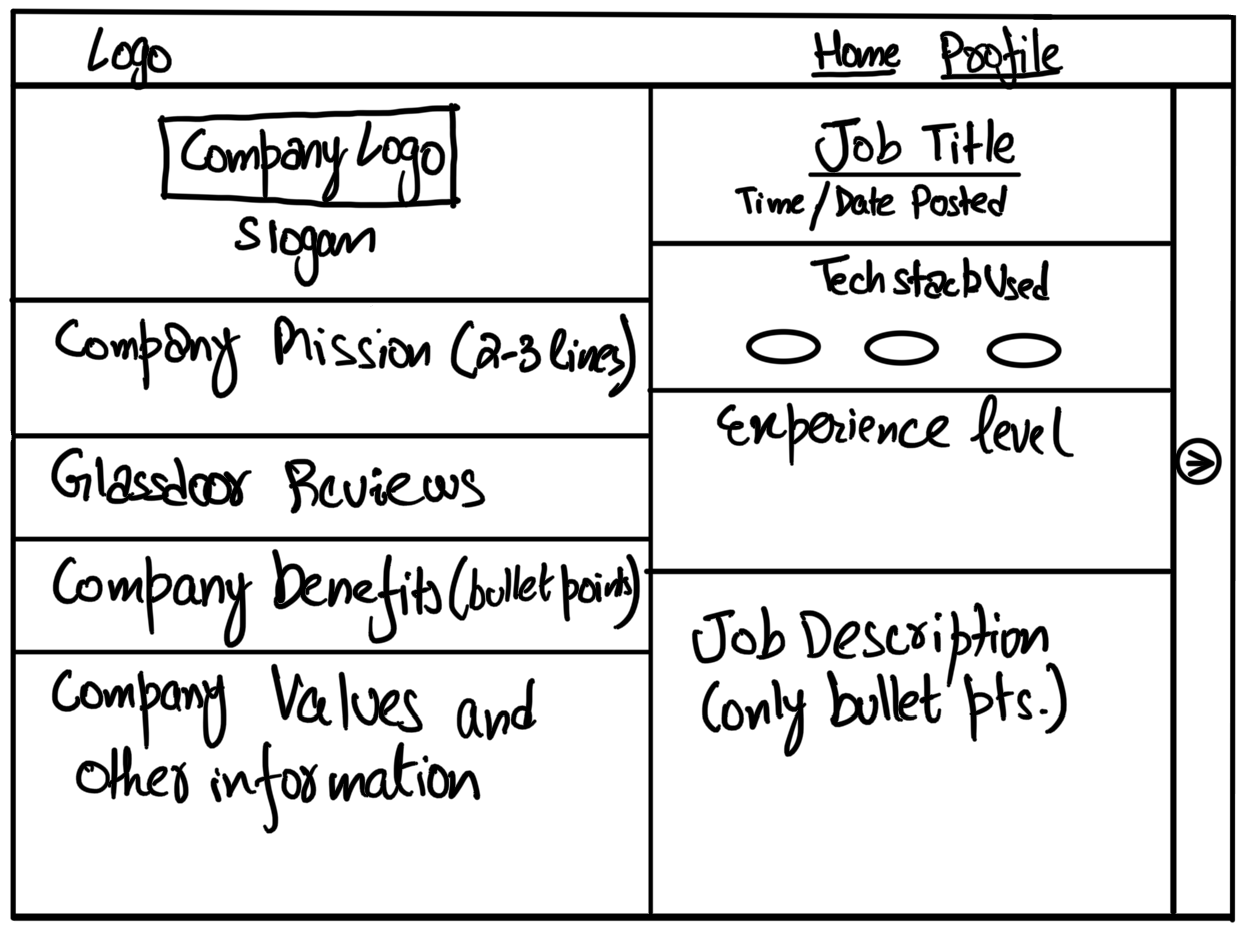
\includegraphics[width = 140mm]{Figures/lowfidelityprototype.png}
    \decoRule
    \caption[Low-Fidelity Prototype of the web app]{Low-fidelity Prototype of a job posting on the app}
    \label{fig:Low fidelity Prototype of a job posting on the app}
\end{figure}

These were the main reasons and justification behind building this web app. 

\newpage
\section{Current Applications}
There are many popular job search engines on the internet, and below is the current research on the most used ones \parencite{Reference1}.

\subsection{Indeed}
As of September 2021, Indeed is the number one job site in the world \parencite{Reference2} and is the reason why this research needs to begin with this web-app. Indeed's statistics show that during the period of April-September 2022, there were about 300 million unique visitors on the platform each month \parencite{Reference3}. Indeed has become this popular due various reasons one of which was due to its correct entry to the market in 2004 before which applying to jobs mostly happened offline and because it was free to use. The success of Indeed is due to two main reasons: 
\begin{itemize}
    \item It's Fast and Free for employers: About 43 percent of job openings are filled within the first 30 days, according to a new report from Indeed and the Centre for Economic and Business Research (CEBR). And the 57 percent of job openings that aren’t filled during that first month will likely remain unfilled for three months or more \parencite{Reference7}. Using Indeed is also free of cost so business owners on a tight budget don't need to spend a penny to post a job on Indeed. 
    \item Just Jobs for applicants: Going into the Indeed website, even if you're not logged in, shows the user just two fields to enter: "What?" and "Where?". Entering those will provide the user with all the jobs related. This helps users find the job they want quickly without having to go through all the trouble of logging in before looking for a job like it's competitors like LinkedIn, GlassDoor, etc. 
    \begin{figure}
        \noindent
        \centering
        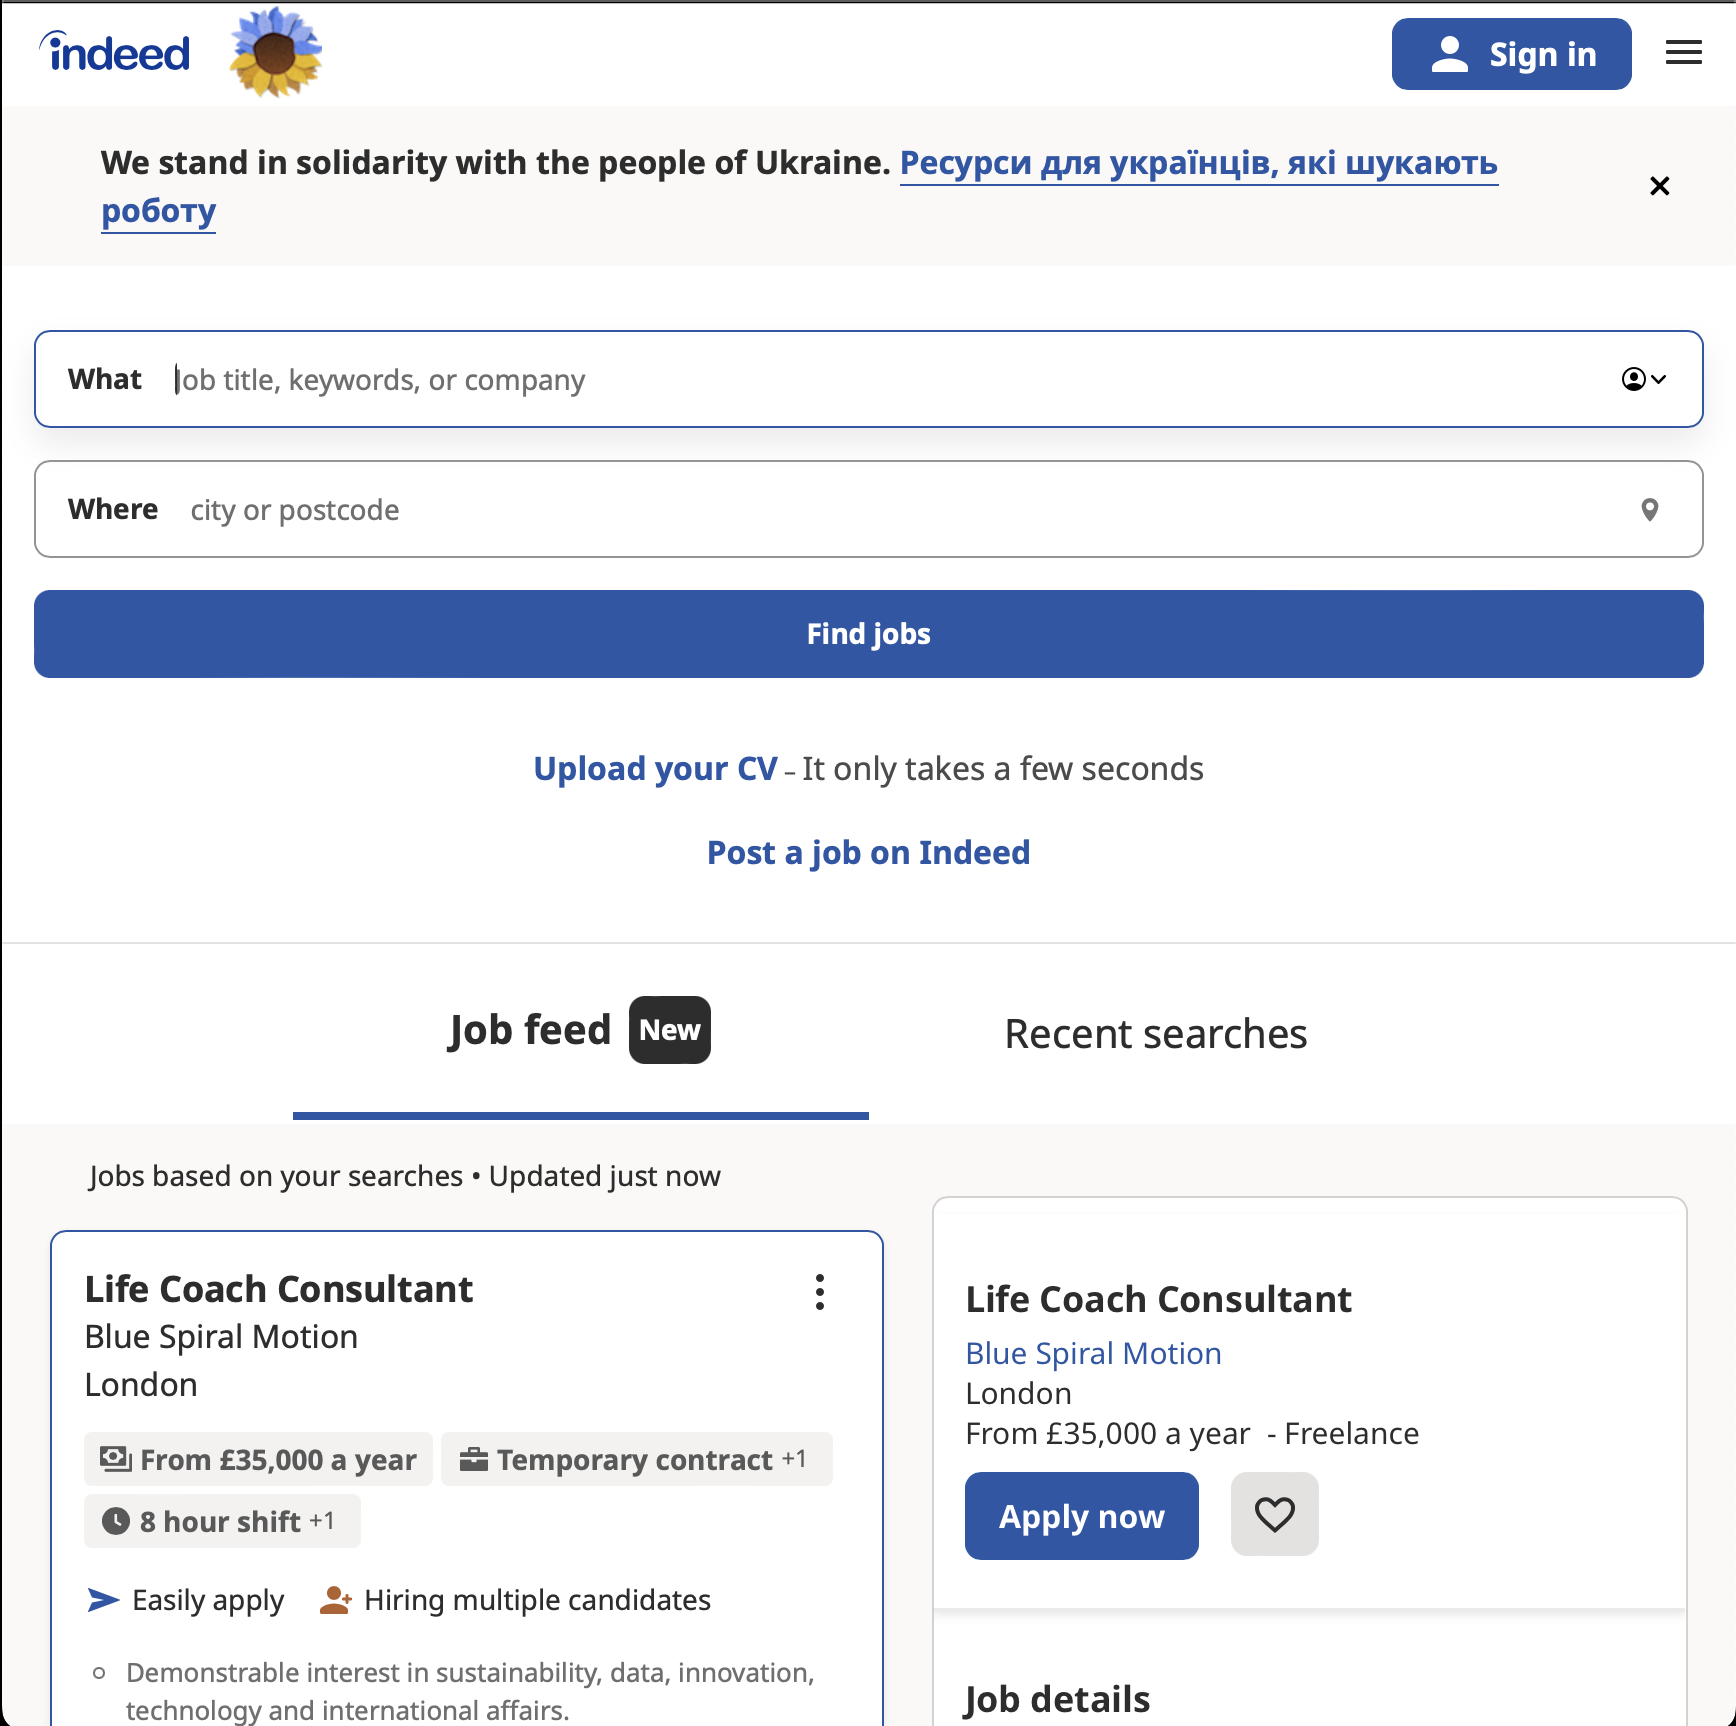
\includegraphics[width = 140mm]{Figures/IndeedHomepage.png}
        \decoRule
        \caption[Indeed's Homepage]{The Homepage of Indeed as of November 2022}
        \label{fig:Indeed Homepage}
    \end{figure}
\end{itemize}

So where does Indeed get it wrong? The main problem with the website is that it is overloaded with jobs. Just searching for a job will provide the user with an enormous list often in the tens of thousands vaguely relevant to their skill set and interests. It's clear to see that Indeed favours quantity over quality. Going by the reviews \parencite{Reference8} on multiple websites, it's clear to see that the users are generally dissatisfied with Indeed. Indeed has a rating of 1.5 on Trustpilot with 4,559 reviews as of November 2022 \parencite{Reference9}. It's clear to see that most users are not happy with the most used job search engine.

\subsection{LinkedIn}
Currently having over 875 million people \parencite{Reference10}, LinkedIn is one of the best places to start networking and reaching out to professionals of different ages and backgrounds related to your career. LinkedIn is a great place to follow different companies a user is interested in and see what they are up to, as well as create a profile for recruiters to look at when they apply for a job. 

However, due to all this networking, LinkedIn is considered more of a social media platform than a job board. This explains why users are redirected to their feed rather than LinkedIn's job search page when they log in to LinkedIn. LinkedIn is also considered the "new Facebook" with tools such as reacting to different posts on your feed like Facebook. LinkedIn is said to be "morphed from a CV Resource to a social media hub" \parencite{Reference14}. An article from the Guardian considers maintaining their LinkedIn page the equivalent of "cleaning their cutlery drawers or wiping down light bulbs – you do it irregularly and perfunctorily because someone told you to, not because there is any obvious benefit." \parencite{Reference11}. Multiple articles suggest that users use LinkedIn because "someone told them to" \parencite{Reference12}. Searching for jobs, on the other hand, is another story. A statistic shows that only 41\% of LinkedIn users thought LinkedIn helped them discover potential job opportunities \parencite{Reference13}. 

What is LinkedIn used for, then, if not for jobs? LinkedIn is considered one of the best tools for networking. It is a great tool to keep in touch with old colleagues and connect with new ones as you go through your professional career, but the future of LinkedIn is not painting an incredible picture for the job seeker.

\begin{figure}
    \noindent
    \centering
    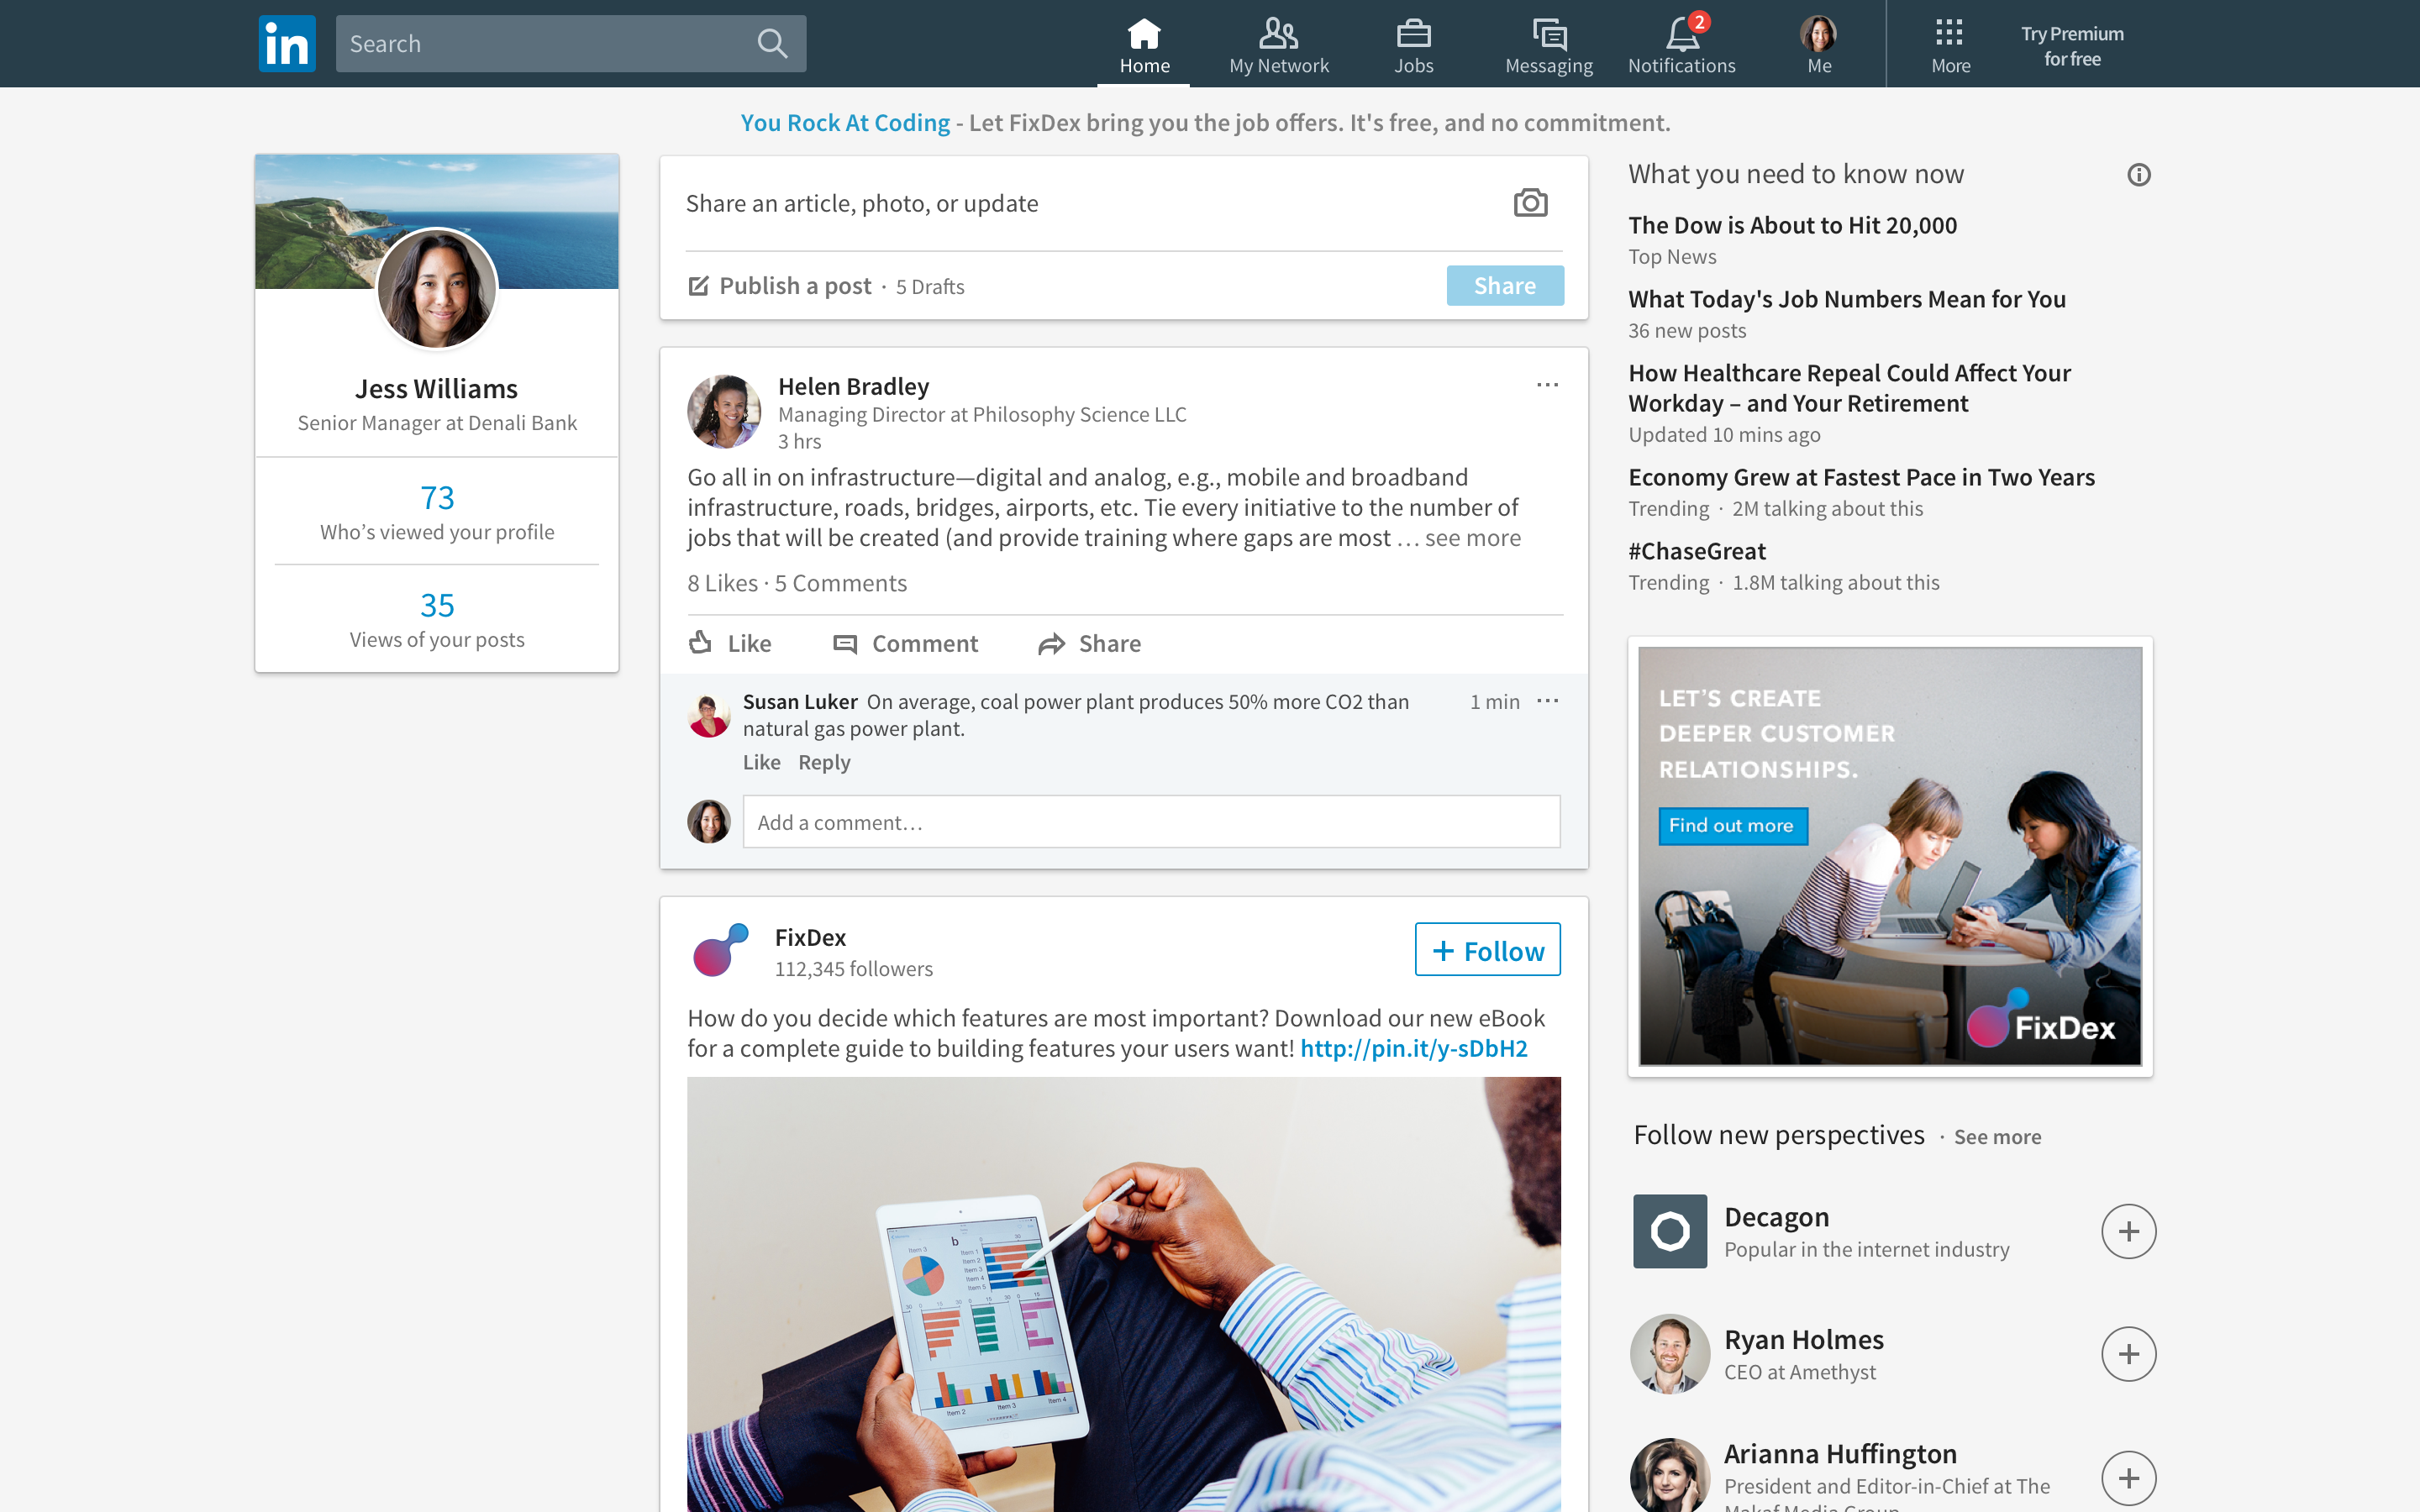
\includegraphics[width = 140mm]{Figures/LinkedInHomepage.png}
    \decoRule
    \caption[LinkedIn's Feed]{The Homepage of LinkedIn as of November 2022}
    \label{fig:LinkedIn Homepage}
\end{figure}

\newpage
\subsection{CareerBuilder}
CareerBuilder is another job search engine that resembles Indeed in several ways. CareerBuilder's homepage has the same two questions (What? and Where?) as Indeed's; however, where it does not resemble Indeed is the price. While Indeed is free to post jobs and look for them, CareerBuilder charges a hefty £349 for their cheapest lite tier, which includes 10 Resume Actions for a day limit \parencite{Reference15}. CareerBuilder does not have any free tier for employers, and as a reason, it is only in the interest of companies which are in a hiring surge or large enough to need hires regularly. With a rating of just 1.48 stars, it is clear that employers and employees alike do not seem to like the product. Users reported getting much spam after registering with CareerBuilder \parencite{Reference16}.

\begin{figure}
    \noindent
    \centering
    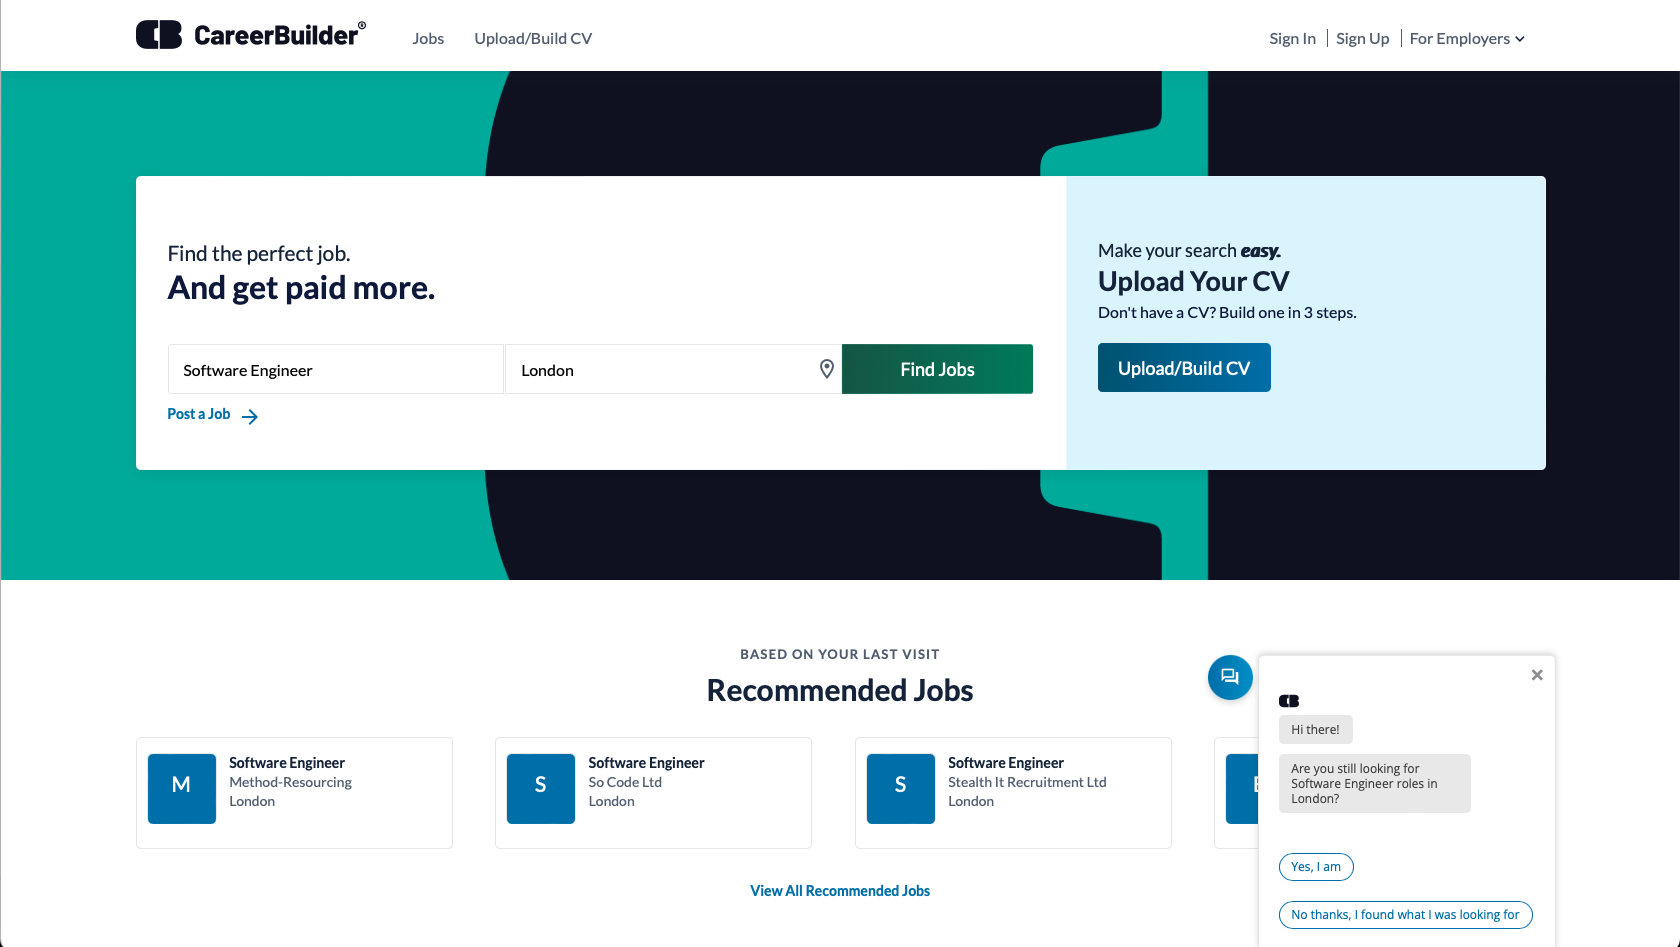
\includegraphics[width = 140mm]{Figures/CareerBuilderHomepage.png}
    \decoRule
    \caption[CareerBuilder's Homepage]{The Homepage of CareerBuilder as of November 2022}
    \label{fig:CareerBuilder Homepage}
\end{figure}

\subsection{Glassdoor}
Glassdoor started as a ratings and reviews web app where employees could leave anonymous reviews to employers. Through the years, Glassdoor has grown, and they now offer a job search engine where users can search for jobs using different filters like salary, employee satisfaction, etc. Unlike Indeed and CareerBuilder, users need to register to search for jobs, but it is free to use. In 2018, Glassdoor was acquired by Indeed's parent company for \$1.2bn making them sister companies. As a result, jobs are shared between both platforms. \parencite{Reference17}

While it can now be used as a job search engine, Glassdoor was mainly designed and developed as a ratings and reviews web app; most users use it for just that. Job seekers mostly use Glassdoor to evaluate a company's work environment, salary and other things, not to look for jobs.

\begin{figure}
    \noindent
    \centering
    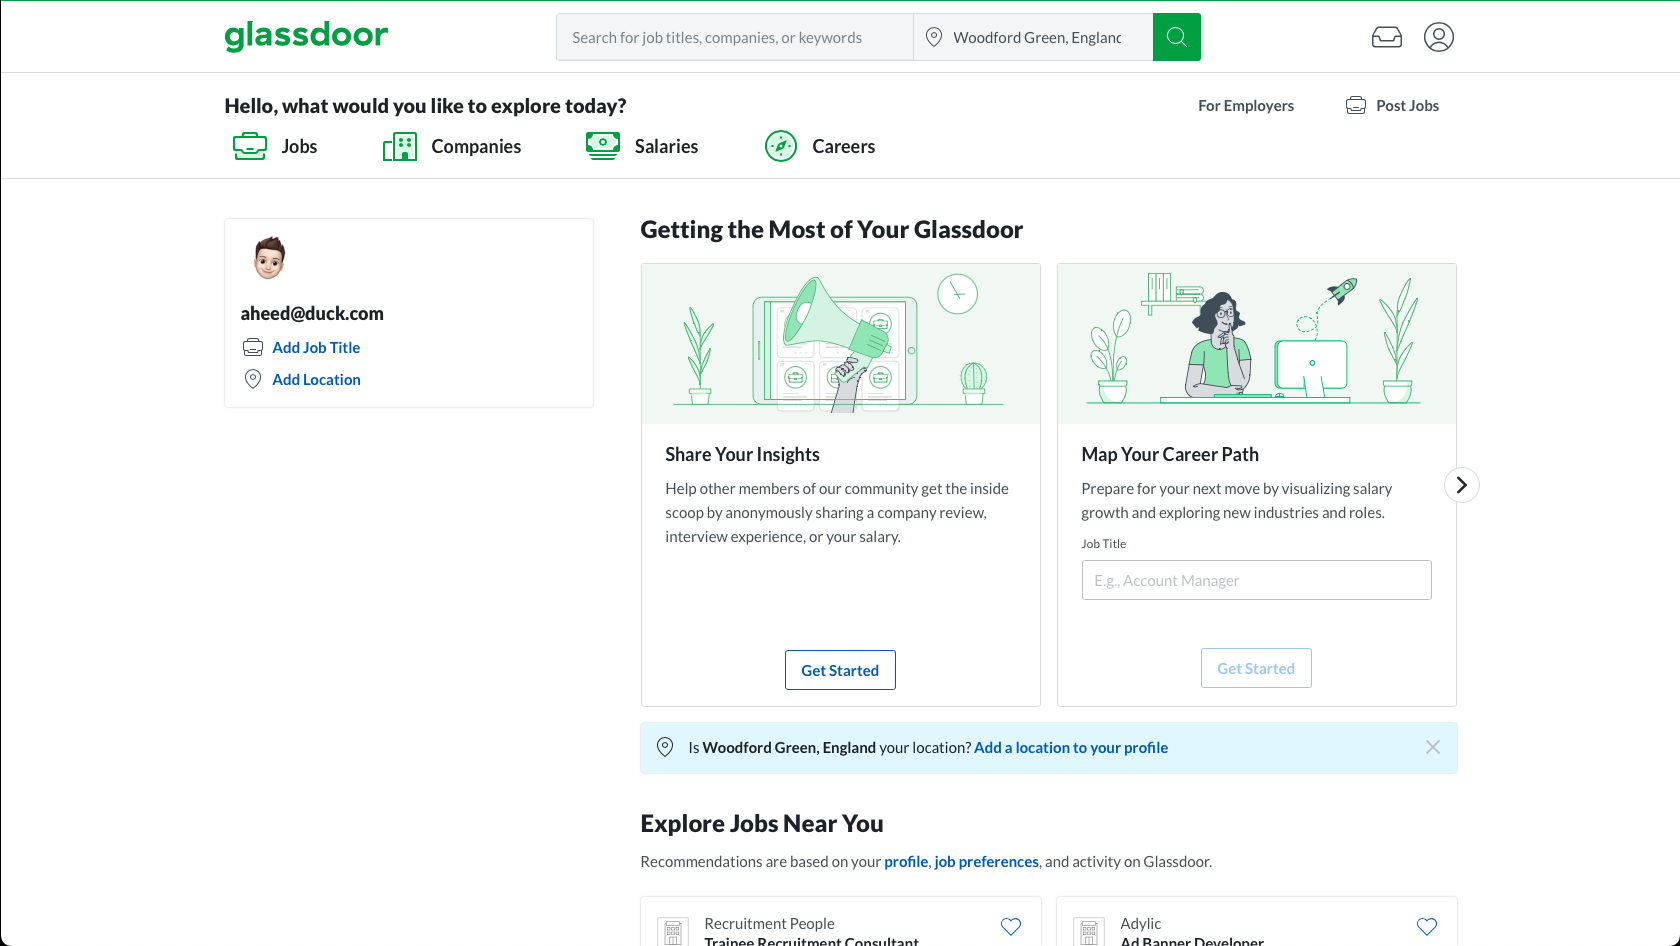
\includegraphics[width = 140mm]{Figures/GlassdoorHomepage.png}
    \decoRule
    \caption[Glassdoor's Homepage]{The Homepage of Glassdoor as of November 2022}
    \label{fig:Glassdoor Homepage}
\end{figure}

\subsection{Existing Tech Job Sites}
Some job boards have been created with the sole purpose of helping applicants in the tech industry find jobs. The most-used among them include: \href{https://itjobpro.com}{IT Job Pro}, \href{https://hired.com}{Hired.com} and \href{https://www.dice.com}{Dice} \parencite{Reference38}. The issue with these applications is the same as mentioned with Indeed. Dice.com, for instance, suffers poor ratings on TrustPilot \parencite{Reference39} and the main thing which echoes through most of the reviews is not receiving any replies and having outdated jobs. 

A user gave the following review for Dice.com: 

"Unable to search easily for remote positions. It requires you use your zip code and then displays jobs in that area, which is not helpful at all to someone working remotely. They do have a check box for "work at home" but you don't see it until you've performed your search. 

This is 2020 - every IT job site should offer an easy to find/use Remote Only option."

This also made it clearer that people in the in the tech industry want to have options filter out their jobs based on how they want to work and this is asked in the questionnaire to help applicants find the right job.

\section{How will this web app be better than the competition?}
Based on the Research on the current applications in the market, this web app will have the following functionalities which will make it better then the products currently in the market for applicants and employers.

\begin{enumerate}
    \item To match applicants with job postings, applicants will be required to fill in a short questionnaire. This will include basic questions which will help match users to job postings. Some sample questions included will be: What is your minimum salary expectations, Do you require a visa to work in the UK?, Which working model do you prefer: Hybrid, In office or at Home?, What tech-stack you want to work with, etc. Answering these questions will help applicants find exactly the job matched they want to see without spending hours creating a resume and answering job-specific questions or going through the entire job description to find information like the tech-stack used in the role.
    \item A redesigned UI will be created which contains one job per screen. About the job and the role's description will be kept on the right hand side of the page and the company description, values will be kept on the left hand side. Keeping these separate in pages, will further help applicants find the information they are looking for.
    \item Applicants will get a reply back saying that their application was unsuccessful if they do not receive a reply from the company within fourteen days of applying.
    \item To make sure there are no outdated jobs, job postings will be required to be set as still active every fourteen days by the employer. If a job hasn't been set active, it will be automatically removed from the web app.
\end{enumerate}

Employers will prefer using this application because of the following features:

\begin{enumerate}
    \item Employers will prefer to use this application as they will know that their ad is only being shown to someone with the same matches which will make finding the ideal applicant earlier. Time taken to hire an employee is at a record-high with average time to hire a candidate is approximately a month \parencite{Reference37}. This is mostly because everyone is shown every role on a traditional job searching website. Searching a Software Engineer role on a traditional website shows you all roles which use C\#, Java or even ML programming languages which makes it harder to find the right applicant. 
    \item Employers will be able to showcase their company like in no other job posting application. They will be able to showcase company brand and culture through your job postings to attract top talent.
    \item Employers will have access to analytics and data on their job postings, including how many views and applications each posting received.
    \item Employers will be given the option to take down the job, to edit the job posting and to add more than just one job on the platform.
\end{enumerate}

The above are the functionalities this web app will have to make it better than the competition currently in the industry with more functionalities which will be added with time.

\section{Tools and Technologies}
During the implementation stage of this web app, various tools and technologies were used. Below is a list of tools and languages with which the development stage was done. As many of these tools were completely new to me, additional knowledge about them was gained through online courses through Udemy \parencite{Reference25}, Coursera \parencite{Reference26} or other websites. 

The language used to build this software are: React, HTML, SASS and Firebase. The reason why these languages are chosen is because:

\begin{itemize}
    \item \textbf{React:} \parencite{Reference20}
    \begin{itemize}
        \item Reusable Components: One of the main advantages of React is that you can reuse components. It saves much time as you do not have to code the same feature again, and you can reuse them.
        \item Speed: React minimises DOM changes, making it highly efficient and providing excellent performance to users.
        \item Easy to Test: React provides its testing library, making it really easy to test its components.
        \item Familiarity: React is very similar to JavaScript, which makes it familiar to Native JavaScript.
    \end{itemize}
    \item \textbf{HTML5:} \parencite{Reference21}
    \begin{itemize}
        \item HTML code will be used inside react components to make them reusable.
        \item HTML ensures the proper formatting of text and images for any Internet browser.
    \end{itemize}
    \item \textbf{SASS:} \parencite{Reference22}
    \begin{itemize}
        \item SASS contains all the CSS features and more features not present in CSS, making it a good choice for developers to use.
        \item SASS offers variables; you can shorten your code by using variables. It is a great advantage over conventional CSS.
    \end{itemize}
    \item \textbf{Firebase:} \parencite{Reference24}
    \begin{itemize}
        \item Authentication SDK using Firebase is very easy, and many features like "Sign in using Google" or "Sign in with Apple" can be used easily through Firebase.
        \item Firebase provides a free tier with many features perfect for this web app, including 100 simultaneous connections fit for an MVP of this product.
    \end{itemize}
\end{itemize}

To use all the languages and tools, IntelliJ IDEA Ultimate Edition \parencite{Reference23} was fit used as it was fit for these languages. It also contains countless extensions with which using these languages becomes easy. 

Version Control is essential to all developers, even when you are working alone. The peace of mind you have when you know a working backup if safe is essential for a developer. As I was working alone while building this application, online version control was not necessary and as a result, this project was version controlled on my personal computer. Version control helped keep track of changes and revert back to old implementation if a serious bug was encountered.

Agile methodologies were used during the development stage. The work was completed in small increments. Testing was done regularly to make sure this web application met the stakeholder's needs. Sprint boards were used to help keep track of the progress of the development of software as well as any bugs which popped up during the development of this app.

\section{Summary}
It was beneficial to research existing applications on the internet that job seekers use to look to begin or further their careers. It helped identify the key features of what this app should have to make it one of the best in the market for tech jobs. The main points for this application that should stand out were:

\begin{itemize}
    \item \textbf{No endless scrolling:} This app will show jobs designed loosely like a pamphlet where every bit of information is in bold and in front, and users will have the option to apply for the job or skip to the next one (See Figure \ref{fig:Low fidelity Prototype of a job posting on the app}). 
    \item \textbf{A reply back:} A poll suggests that 62\% of applicants spend at least 30 minutes on their application, and 38\% spend up to 30 minutes on an application. \parencite{Reference18}. Every applicant who spends time sending an application for a job deserves a reply from companies. This app, in addition to sending an email when applying for a job, will send one as soon as the job is marked as filled by the recruiter or taken down from the platform.
    \item \textbf{Reinventing job descriptions:} Job descriptions need to be rethought. Going through job descriptions in tech is a nightmare. The need to scroll down all about the company's profile to find what tech stack they use or what the level of the job applicant should be (entry-level, mid-level or senior level). This app will solve it by keeping separate tags below the job title, which should point out the technologies/languages the company uses. (See Figure \ref{fig:Low fidelity Prototype of a job posting on the app})
    \item \textbf{No Outdated jobs:} One of the main criticisms in the online job search industry is that they include many outdated jobs. Job Crop should be different in this regard. Jobs will not be shown on the platform after fourteen days. If the job is still open and the recruiters have yet to find a candidate, they will get an option to keep the job on the platform for another fourteen days if they wish to do so.
    \item \textbf{Only Jobs in tech:} Job search engines like LinkedIn have strayed away from being what a job search engine should be: Just jobs. This app will be built on the foundation that users would come to this app for just one thing: A job in the tech industry.
\end{itemize}